\documentclass[tikz,border=10pt]{standalone}
\usepackage{tikz}
\usepackage{xcolor}
\usetikzlibrary{shapes,arrows,positioning,calc,fit}

\definecolor{inputcolor}{RGB}{225,245,255}
\definecolor{stemcolor}{RGB}{255,249,196}
\definecolor{branchcolor}{RGB}{248,187,208}
\definecolor{physicscolor}{RGB}{209,196,233}
\definecolor{outputcolor}{RGB}{200,230,201}

\begin{document}
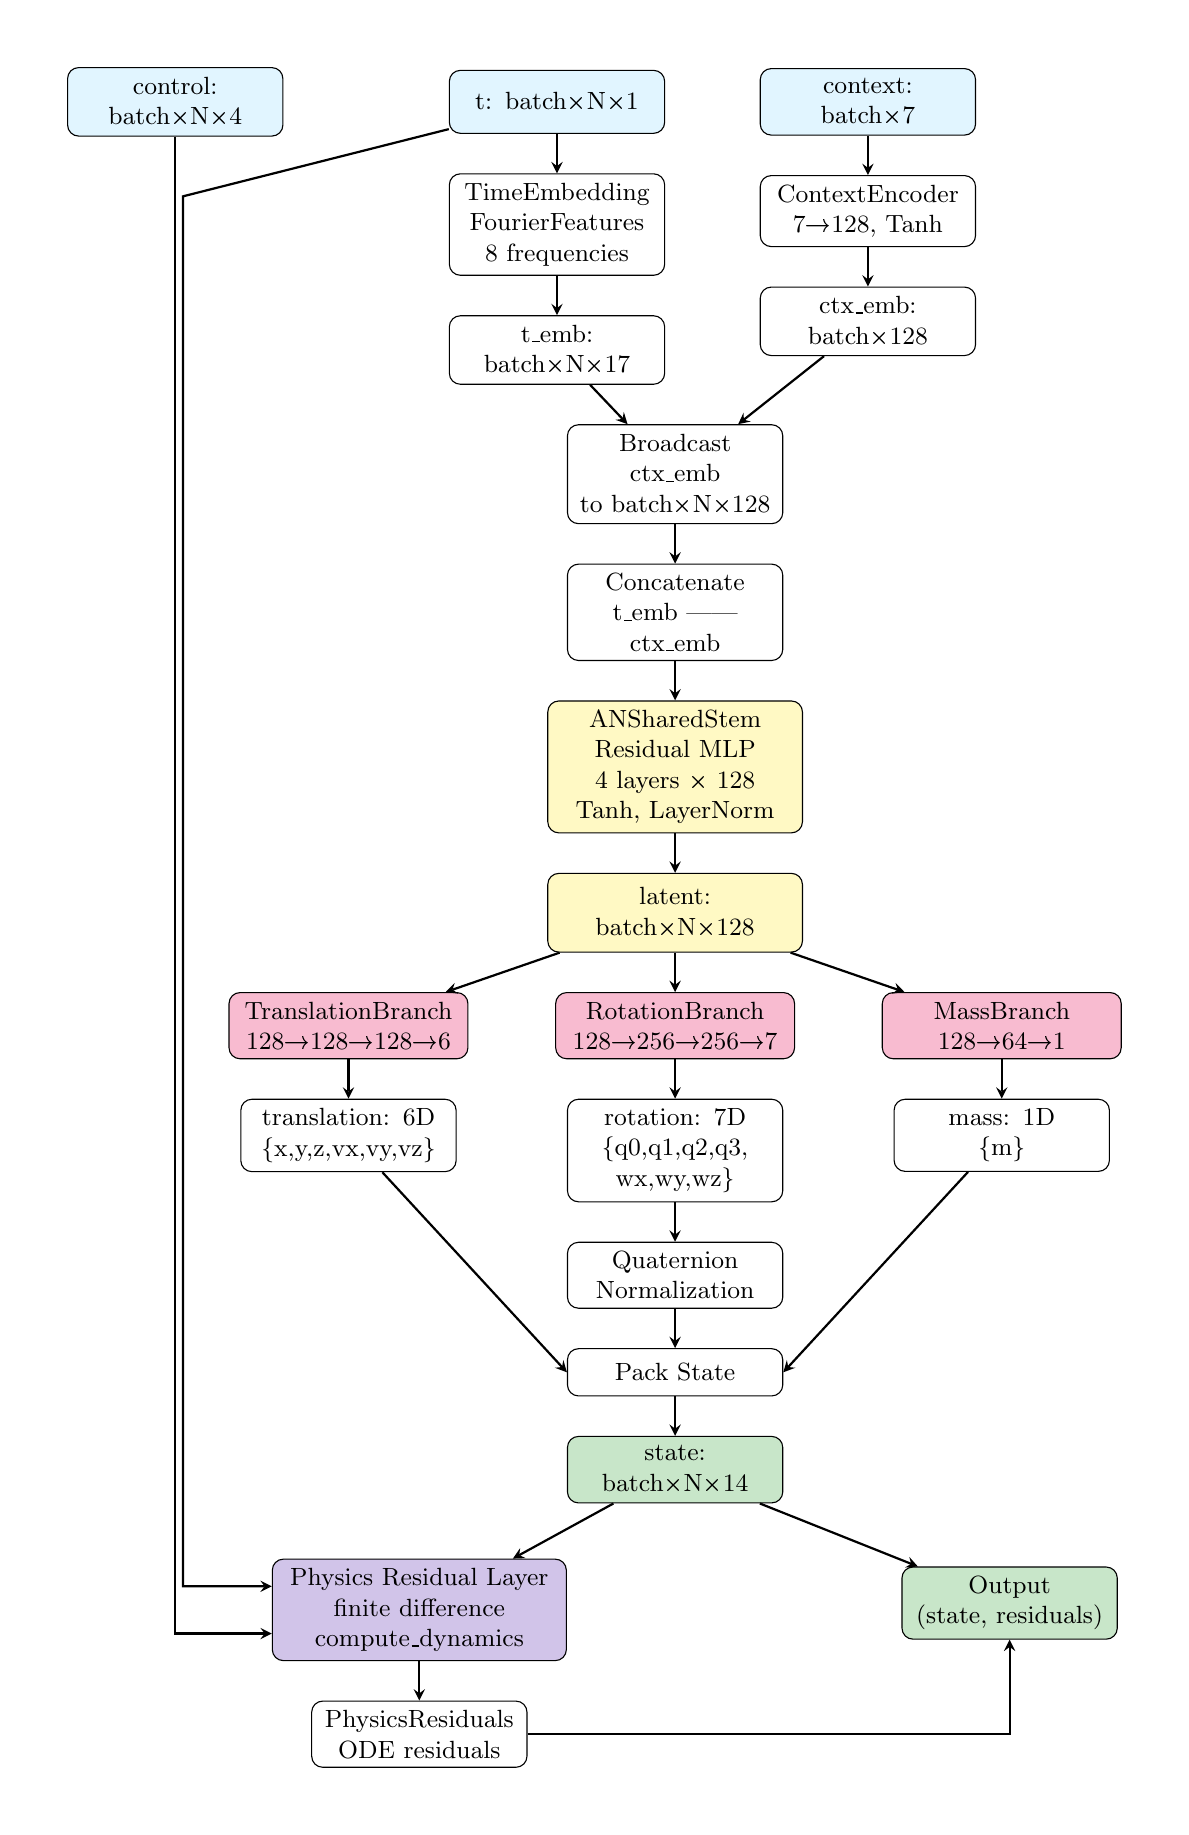
\begin{tikzpicture}[
    node distance=0.5cm and 1.2cm,
    remember picture,
    every node/.style={font=\small},
    input/.style={rectangle, rounded corners, fill=inputcolor, draw=black, text width=2.5cm, text centered, minimum height=0.8cm},
    stem/.style={rectangle, rounded corners, fill=stemcolor, draw=black, text width=3cm, text centered, minimum height=1cm},
    branch/.style={rectangle, rounded corners, fill=branchcolor, draw=black, text width=2.8cm, text centered, minimum height=0.8cm},
    physics/.style={rectangle, rounded corners, fill=physicscolor, draw=black, text width=3cm, text centered, minimum height=0.8cm},
    output/.style={rectangle, rounded corners, fill=outputcolor, draw=black, text width=2.5cm, text centered, minimum height=0.8cm},
    process/.style={rectangle, rounded corners, fill=white, draw=black, text width=2.5cm, text centered, minimum height=0.6cm},
    arrow/.style={->, >=stealth, thick}
]

% Input nodes - placed at top horizontally
\node[input] (A) {t: batch×N×1};
\node[input, left=of A, xshift=-0.9cm] (Q) {control: batch×N×4};
\node[input, right=of A] (C) {context: batch×7};

% Embedding layer - positioned below inputs
\node[process, below=0.5cm of A] (B) {TimeEmbedding\\FourierFeatures\\8 frequencies};
\node[process, below=0.5cm of C] (D) {ContextEncoder\\7→128, Tanh};

\node[process, below=of B] (E) {t\_emb: batch×N×17};
\node[process, below=of D] (F) {ctx\_emb: batch×128};

\node[process, below=of E, xshift=1.5cm] (G) {Broadcast ctx\_emb\\to batch×N×128};
\node[process, below=of G] (H) {Concatenate\\t\_emb || ctx\_emb};

% Shared stem
\node[stem, below=of H] (I) {ANSharedStem\\Residual MLP\\4 layers × 128\\Tanh, LayerNorm};
\node[stem, below=of I] (J) {latent: batch×N×128};

% Mission branches
\node[branch, below left=0.5cm and 1.0cm of J] (K1) {TranslationBranch\\128→128→128→6};
\node[branch, below=of J] (K2) {RotationBranch\\128→256→256→7};
\node[branch, below right=0.5cm and 1.0cm of J] (K3) {MassBranch\\128→64→1};

% Branch outputs
\node[process, below=of K1] (L1) {translation: 6D\\\{x,y,z,vx,vy,vz\}};
\node[process, below=of K2] (L2) {rotation: 7D\\\{q0,q1,q2,q3,\\wx,wy,wz\}};
\node[process, below=of K3] (L3) {mass: 1D\\\{m\}};

% Processing
\node[process, below=of L2] (M) {Quaternion\\Normalization};
\node[process, below=of M] (N) {Pack State};
\node[output, below=of N] (O) {state: batch×N×14};

% Physics layer
\node[physics, below left=1.2cm and 1.5cm of O, text width=3.5cm, xshift=1.5cm, yshift=0.5cm] (P) {Physics Residual Layer\\finite difference\\compute\_dynamics};
\node[process, below=of P] (R) {PhysicsResiduals\\ODE residuals};

% Final output
\node[output, below right=0.8cm and 1.5cm of O] (S) {Output\\(state, residuals)};

% Arrows
\draw[arrow] (A) -- (B);
\draw[arrow] (B) -- (E);
\draw[arrow] (C) -- (D);
\draw[arrow] (D) -- (F);
\draw[arrow] (E) -- (G);
\draw[arrow] (F) -- (G);
\draw[arrow] (G) -- (H);
\draw[arrow] (H) -- (I);
\draw[arrow] (I) -- (J);
\draw[arrow] (J) -- (K1);
\draw[arrow] (J) -- (K2);
\draw[arrow] (J) -- (K3);
\draw[arrow] (K1) -- (L1);
\draw[arrow] (K2) -- (L2);
\draw[arrow] (K3) -- (L3);
\draw[arrow] (L2) -- (M);
\draw[arrow] (L1) -- (N.west);
\draw[arrow] (M) -- (N);
\draw[arrow] (L3) -- (N.east);
\draw[arrow] (N) -- (O);
\draw[arrow] (O) -- (P);
% Arrows from inputs to physics layer - route around sides to avoid crossings
% Separate endpoints on P.west by using different y-positions
\draw[arrow] (A) -- ++(-4.75cm,-1.2cm) |- ([yshift=0.3cm]P.west);
\draw[arrow] (Q.south) -- ++(0,0) |- ([yshift=-0.3cm]P.west);
\draw[arrow] (P) -- (R);
\draw[arrow] (O) -- (S);
\draw[arrow] (R) -| (S);

% Add padding to ensure everything fits within the bounding box
\useasboundingbox ([shift={(-0.5cm,-0.5cm)}]current bounding box.south west) rectangle ([shift={(0.5cm,0.5cm)}]current bounding box.north east);

\end{tikzpicture}
\end{document}
